\documentclass{article}
\usepackage{amsmath}
\usepackage{amsfonts}
\usepackage{amsthm}
\usepackage{amsmath}
\usepackage{mathtools}
\usepackage{url}
\newcommand{\abs}[1]{\left\lvert#1\right\rvert}
\begin{document}

\title{An Application of Hahn-Banach theorem in Separation of Two Disjoint Point Sets in Two Dimensional Space}

\maketitle


%
\begin{abstract}
	In this article  we give another approach of linear separation of two disjoint data sets instead of SVM (supporter vector machine). We use famous Hahn-Banach theorem and its
	proposition, strict separation theorem to derive a linear separator in two dimensional case. The construction of linear separator
	can be done by our precise analysis of Minkowski functional of convex hull, which is derived from Minkowski difference of two
	convex hulls of data sets. Our method gives a deterministic approach to linear separator, instead of iterative method used in
	SVM.
\end{abstract}

\section{Introduction}
\label{sec:intro}
Hahn-Banach theorem is a well known mathematical tool for functional analysis, In a word, it states that given a sublinear functional
$p$ on space $E$, and a linear functional $\ell$ on subspace $V$, which satisfies $\ell\leq p$, we can extend the functional $\ell$ to linear
functional $\tilde{\ell}$ on whole space $E$ and still satisfies the inequality. A direct consequence is the following: Given two disjoint
sets $A$ and $B$, chosen any points $a_0\in A$ and $b_0\in B$, we construct set $C$:
\begin{equation*}
	C=\{y_0:y_0=a-b+b_0-a_0,a\in A, b\in B\}
\end{equation*}
Considering Minkowski functional $p_C$ of set $C$, it guarantees that $p_C(x)\leq 1$ for $x\in C$ and $p_C(x)>1$ for $x\notin C$. If we
let $\ell(b_0-a_0)=p_C(b_0-a_0)$ and extend $\ell$ on whole space $\mathbb{R}^d$ to $\tilde{\ell}$ with restriction $\ell\leq p_C$, the following inequality will
hold:
\begin{equation*}
	\max_{a\in A}{\tilde{\ell}(a)}\le\min_{b\in B}{\tilde{\ell}(b)}
\end{equation*}
By computing the two sides of inequality, $\tilde{\ell}(x)=\gamma$ will separate two sets where:
\begin{equation*}
	\gamma\in[\max_{a\in A}{\tilde{\ell}(a)},\min_{b\in B}{\tilde{\ell}(b)}]
\end{equation*}
and it gives mathematical foundation of possibility of separating two disjoint sets by a hyperplane~\cite{bertsekas2009convex}. We will 
give details of the proof of above statements in section~\ref{sec:proof}. However, there are some existence proof skills in proof 
of the theorem~\cite{stein2011functional}. Thus we cannot derive the separating hyperplane directly from the proof. \par

Due to the work of Corinna Cortes and Vapnik, SVM gives a gradient approach to construct the separating hyperplane
~\cite{cortes1995support}. And it becomes the most popular mechanism for solving classification problem~\cite{bishop2006pattern}. The 
current usage of sub-gradient method for SVM without kernel needs $O(ndT)$ time, for n examples, d dimensions, T steps~\cite{9520}. The 
shortage of SVM is it does not guarantee we get the solution in a given time. \par

In this article, we review the proof of Hahn-Banach theorem, and in section~\ref{sec:bounds analysis} prove that the key functional, 
Minkowski functional is piecewise linear convex function by constructing the analytical form of Minkowski functional, when it is a 
functional of a convex polygon. The construction of analytical form cannot be done in general cases. Furthermore, we show that the 
minimum of Minkowski functional on a convex polygon can be computed directly once we have the convex hull, without using any gradient 
method.\par

We conclude that two disjoint data sets, separator in linear separation problem can be easily constructed using a convex polygon $K$ 
obtained from Minkowski difference of two data sets with the help of Minkowski functional. And the minimum of Minkowski functional makes construction steps 
possible and quickly be done in practice, instead of using any gradient method like SVM.
In section~\ref{experiment}, we give three results in 2D case. We show that for two disjoint sets, our separator can separate two sets accurately. And our
separator behaves well even when two sets have a little of intersection. Our experiments is in two dimensional case, but the algorithm is expected to be used 
in any dimensional space.\par

From a higher perspective, this functional approach is using Minkowski functional of convex hull related to data set measures the whole data space.\par

% section 2
\section{Preliminaries}
In the following sections, $Conv(A)$ denotes the convex hull of point set $A$. $A\setminus B$ denotes the set difference of A and B. 
$span\{x_0,x_1,\dots,x_d\}$ denotes the set of all finite linear combinations of $x_0,x_1,\dots,x_d$. $\abs{\cdot}$ denotes 2-norm.\par

\emph{Definition 2.1} (Minkowski difference). Given a vector space $V$ and two point sets $A$ and $B$ in $V$, the Minkowski difference $A\ominus B$ is 
defined as:
\begin{equation*}
	A\ominus B=\{a-b\mid a\in A\text{ and }b\in B\}
\end{equation*}
Without proof here, we use the fact that
\begin{equation}\label{eq:Minkowski sum}
	Conv(A\ominus B)=Conv(A)\ominus Conv(B)
\end{equation}
The proof of above equation is easy and can be found in~\cite{625624}.\par

\emph{Definition 2.2} (sublinear functional). Given a vector space $V$ and a functional $P:V\to\mathbb{R}$, we call $P$ is a
sublinear functional if:
\begin{equation}\label{property:sublinear}
	\left\{\begin{aligned}
		 & P(av)=aP(v),                  & \mbox{if $a \geq 0$ and $v\in V$} \\
		 & P(v_1+v_2)\leq P(v_1)+P(v_2), & \mbox{if $v_1,v_2\in V_0$}
	\end{aligned}
	\right.
\end{equation}
\emph{Definition 2.3} (Minkowski functional). Given a vector space $V$ and a non empty set $K$ including $0$, and $0$ is not on the boundary of set $K$. 
For $v \in V$ define:
\begin{equation*}
	p_K(v)=\inf_{r>0}\{r: v/r \in K\}
\end{equation*}
and functional $p_K$ completely characterized $K$ in that
\begin{equation*}
	p_K(v)\leq 1\qquad if~and~only~if~v \in K
\end{equation*}
One important property of Minkowski functional is a sublinear functional~\cite{stein2011functional}.\par



\emph{THEOREM 2.4} (Hahn-Banach Theorem).
\emph{Suppose $V_0$ is a linear subspace of $V$ and $p$ is a sublinear functional on $V$, and that we are given a linear functional $\ell$ on $V_0$ that
	satisfies
	\begin{equation*}
		\ell(v)\le p(v),\qquad ~for~all~v \in V_0
	\end{equation*}
	Then $\ell$ can be extended to a linear functional $\tilde{\ell}$ on $V$ that satisfies
	\begin{equation*}
		\tilde{\ell}(v)\le p(v),\qquad~for~all~v \in V
	\end{equation*}
}\par
\emph{THEOREM 2.5} (Strict Separation Theorem).
\emph{Given a vector space $V$, and two non empty convex set $A$ and $B$, which satisfy:
	$A\cap B=\emptyset$. Then there is a linear functional $\ell$, and a real number $\alpha\in\mathbb{R}$, s.t.
	\begin{equation*}
		\max_{a\in A}{\ell(a)}<\alpha<\min_{b\in B}{\ell(b)},\qquad a\in A
	\end{equation*}
}
Since our construction of linear separator is based on the proof of theorem 2.4 and 2.5, we will show the proof of theorems in section~\ref{sec:proof}
and analyze some functions in the proof in section~\ref{sec:bounds analysis}.

% section 3
\section{Proofs}
\label{sec:proof}
In this section we will prove theorem 2.4 and theorem 2.5. The procedure of proofs will be used in constructing linear separator.
\subsection{Proof of Theorem 2.4}
\label{subsec:proof HB}
\begin{proof}
	Given $\ell(x_0)$ for subspace $x_0\in V_0$, we select any vector $x_1$ which is in space $V\setminus V_0$ and
	be ready to extend $\ell$ to the subspace $span\{x_0,x_1\}$. We can make a choice for the value of $\tilde{\ell}$ on $x_1$, so as to satisfy
	$\tilde{\ell}(x)\le p(x), \forall x\in V$ if
	\begin{equation*}
		a\tilde{\ell}(x_1)+b\tilde{\ell}(x_0)=\tilde{\ell}(ax_1+bx_0)\le p(ax_1+bx_0),\qquad \forall a,b\in\mathbb{R}
	\end{equation*}
where $\tilde{\ell(x)}=\ell(x)$ for all $x\in V_0$.	If $a=0$, above inequality trivially holds. If $a\neq 0$
	\[
		\left\{
		\begin{array}{ll}
			\tilde{\ell}(x_1)\leq \frac{p(ax_1+bx_0)-b\tilde{\ell}(x_0)}{a},a>0 \\
			\tilde{\ell}(x_1)\geq \frac{b\tilde{\ell}(x_0)-p(ax_1+bx_0)}{-a},a<0
		\end{array}
		\right.
	\]
	Then we get:
	\begin{equation*}
		\tilde{\ell}(w)-p(-x_1+w)\leq\tilde{\ell}(x_1)\leq p(x_1+w')-\tilde{\ell}(w'),\qquad ~\forall w, w'\in V_0
	\end{equation*}
	Since
	\begin{align*}
		\tilde{\ell}(w)+\tilde{\ell}(w')= &\tilde{\ell}(w-x_1+w'+x_1)  \\
		\leq              & p(w-x_1+w'+x_1)     \\
		\leq              & p(-x_1+w)+p(x_1+w')
	\end{align*}
	always holds. The first inequality holds because of $w+w'\in V_0$, The second equality holds because of sublinear property of $p$. The Thus the 
	upper bound of $\tilde{\ell}(x_1)$ is
	\begin{equation}\label{l upper bound}
		\min_{w\in V_0}{\{-\tilde{\ell}(w)+p(w+x_1)}\}
	\end{equation}
	and the lower bound is
	\begin{equation}\label{l lower bound}
		\max_{w'\in V_0}{\{\tilde{\ell}(w')-p(w'-x_1)}\}
	\end{equation}
	We can choose any real number between two bounds as value of $\tilde{\ell}(x_1)$. In practice, we can choose the mean of two bounds as value of $\tilde{\ell}(x_1)$.
	% \begin{equation*}
	% 	$\ell(x_1)=\frac{\sup_{w\in V_0}{(\ell(w)-p(w-x_1)})+\inf_{w'\in V_0}{(-\ell(w')+p(w'+x_1))}}{2}$
	% \end{equation*}
	We can now extend subspace $V_0$ to $span\{x_0,x_1\}$ and letting
	\begin{equation*}
		\tilde{\ell}(\lambda_0x_0+\lambda_1x_1)=\lambda_0\tilde{\ell}(x_0)+\lambda_1\tilde{\ell}(x_1)
	\end{equation*}
	We keep doing above step until $V=V_0$ with $\tilde{\ell}(x)$ mapping $V$ to $\mathbb{R}$
\end{proof}
For easier reading, we omit the difference between the symbol $\tilde{\ell}$ and $\ell$ in following sections. We will keep using symbol $\ell$ after extension.
\subsection{Proof of Theorem 2.5}
\label{subsec:proof separation}
\begin{proof}
	Choose $a_0\in A\text{, }b_0\in B$ which $b_0-a_0$ is not on the boundary of $Conv(A\ominus B)$. Let $x_0=b_0-a_0$. Construct set $C$:
	\begin{equation}\label{def:C}
		C=\{y_0:y_0=a-b+x_0,a\in A, b\in B\}
	\end{equation}
	$C$ has following properties:
	\begin{itemize}
		\item $C$ is convex set, because of equation~\ref{eq:Minkowski sum} and shifting set by $x_0$.
		\item $x_0 \notin C$ and $0\in C$, because of $A\cap B=\emptyset$
		      % \item C is open set.(needs more proof)
		      %\item The Minkowski functional $p_C$ associated with C has sublinear property
		\item $\forall x\in C\text{, }p_C(x)\leq1$, where $p_C$ is Minkowski functional of $C$.
	\end{itemize}
	Since the Minkowski functional $p_C$ is a sublinear functional, by Hahn-Banach Theorem, there exists a linear functional $\ell$, s.t.
	\begin{equation*}
		\ell\le p_C\text{ and }\ell(x_0)=p_C(x_0)> 1
	\end{equation*}
	$p_C(x_0)<\infty$ since $x_0$ is not on the boundary of $Conv(A\ominus B)$.
	Then we can extends functional $\ell(x_0)$ to space $V_0=span\{x_0\}$ by letting $\ell(kx_0)=k\ell(x_0)$. For $k\geq0$, the inequality $\ell\leq p_C$ holds by
	property \eqref{property:sublinear}. For $k<0$, the inequality $\ell\leq p_C$ holds immediately.\par
	For all $x\in C$, we have:
	\begin{equation*}
		\ell(a-b+x_0)\le p_C(a-b+x_0)<1
	\end{equation*}
	We get:
	\begin{equation}\label{gamma bound}
		\ell(a)<\ell(b)+1-\ell(x_0)< \ell(b),\qquad\forall a\in A, \forall b\in B
	\end{equation}
	The last inequality holds because of $\ell(x_0)>1$. Thus:
	\begin{equation*}
		\max_{a\in A}{\ell(a)}<\min_{b\in B}{\ell(b)}
	\end{equation*}
	Thus there exists $\alpha\in\mathbb{R}$ which satisfies:
	\begin{equation*}
		\ell(a)<\alpha<\ell(b), \qquad\forall a\in A,b\in B
	\end{equation*}
\end{proof}
In practice, we can choose $\ell(x_0)=p_C(x_0)$, and extend $\ell$ as procedure of proof in section~\ref{subsec:proof HB}. After extending $\ell(x)$ to entire 
vector space $V$, we select
\begin{equation*}
	\gamma\in \left[\max_{a\in A}{\ell(a)},\min_{b\in B}{\ell(b)}\right]
\end{equation*}
for which hyperplane $\ell(x)=\gamma$
will separate
set $A$ and $B$. In practice, we can choose
\begin{equation}\label{optimal gamma}
	 \gamma=\frac{\max_{a\in A}{\ell(a)}+\min_{b\in B}{\ell(b)}}{2}
\end{equation}
as our optimal $\gamma$.




% section 4
\section{Analysis of two bounds of $\ell(x_1)$}
\label{sec:bounds analysis}
In this section, we will show that if we choose $\ell(x_0)=p_C(x_0)$, the two bounds of $\ell(x_1)$ will be equal, where $C$ is defined as equation \eqref{def:C}.
Since upper bound \eqref{l upper bound} of $\ell(x_1)$ has the same form with lower bound \eqref{l lower bound} except for a minus sign, we only need to analyze
the upper bound and use the same routine on lower bound.\par
We rewrite the function $p_C(x_1+w)-\ell(w)$ as
\begin{equation}\label{eq:f(k)}
	f(k)=p_C(x_1+kx_0)-k\ell(x_0)
\end{equation}
We first prove $p_C(x_1+kx_0)$ is piecewise linear continuous convex function of $k$.
Then we analyze function $f(k)$. We choose $x_1$ orthogonal to $x_0$ for the
sake of easier analysis. %\emph{put proof part at the end of article}

\subsection{Analysis of $p_C(x_1+kx_0)$}
In this part, we will show that $p_C(x_1+kx_0)$ is piecewise linear continuous function of $k$. We denote the point at which the ray in direction of  $x_1+kx_0$ 
intersects polygon as $M$. See (a) in figure~\ref{fig:proof}. Then we set the x-axis in direction of $x_0$ and the y-axis in direction
of $x_1$. The result coordinate system as (b) in figure~\ref{fig:proof}. The coordinate value of $M$ satisfies\par
%, introducing a vertical line from point A to line B:\par

%proof
\begin{figure}%[t]
	\begin{minipage}[b]{1.0\linewidth}
        \centering
        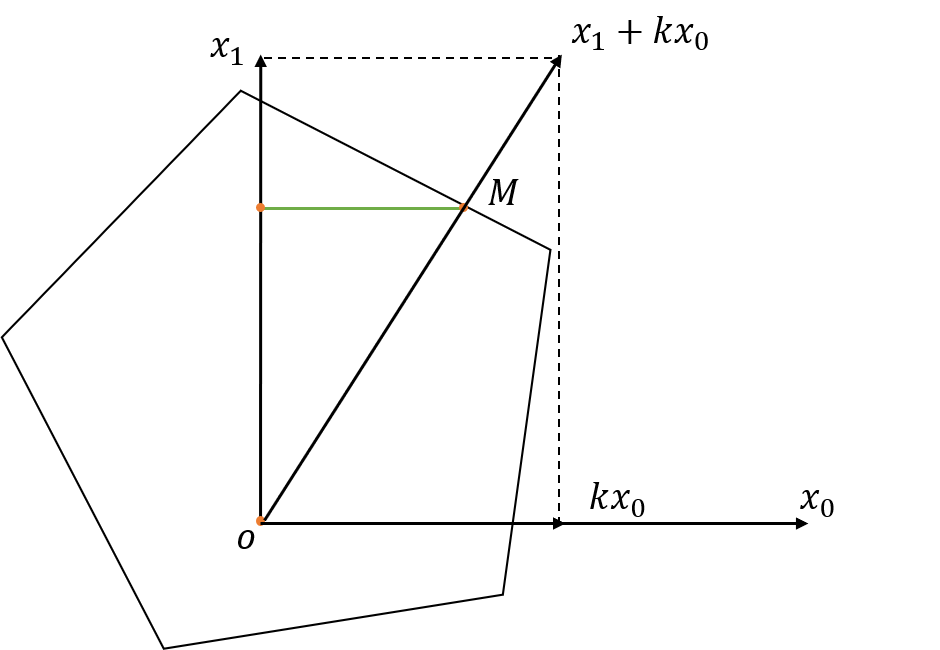
\includegraphics[width=0.6\textwidth]{proof1.png}
		% \centerline{\epsfig{figure=proof1.png,width=8.5cm}}
		%   \vspace{1.5cm}
		\centerline{(a) The intersection of the polygon and the ray}\medskip
	\end{minipage}
	%
	\begin{minipage}[b]{1.0\linewidth}
        \centering
        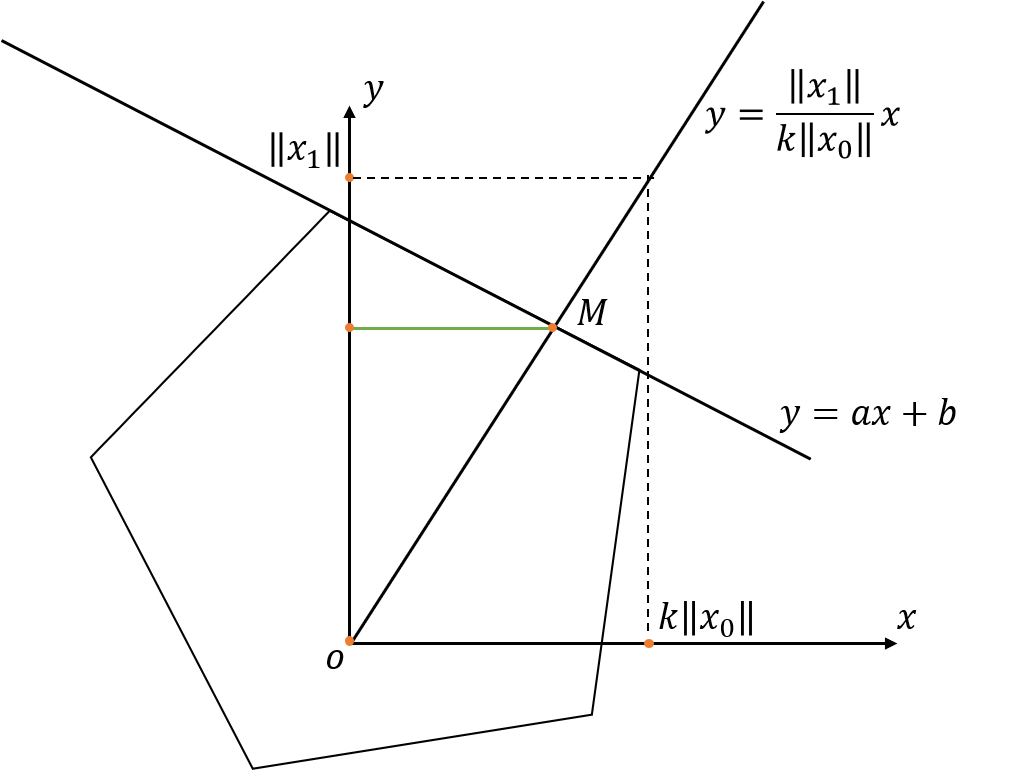
\includegraphics[width=0.6\textwidth]{proof2.png}
		% \centerline{\epsfig{figure=proof2.png,width=8.5cm}}
		%	  \vspace{1.5cm}
		\centerline{(b) The coordinate system and related lines}\medskip
	\end{minipage}

	%
	\caption{The diagram of proof.}
	\label{fig:proof}
\end{figure}

\begin{equation}\label{s}
	\left\{
	\begin{aligned}%
		 y & =ax+b                                        \\
		 y & =\frac{\lVert x_1\rVert}{k\lVert x_0\rVert}x
	\end{aligned}
	\right.
\end{equation}
Solving equation \eqref{s} we get the x-axis component of $M$ is:
\begin{equation*}
	x_M=\frac{bk\abs{x_0}}{-ak\abs{x_0}+\abs{x_1}}
\end{equation*}
By triangle similarity, $p_C(x_1+kx_0)=\frac{k\abs{x_0}}{x_M}$,
we get:
\begin{equation}\label{explicit p}
	p_C(x_1+kx_0)=-\frac{a\abs{x_0}}{b}k+\frac{\abs{x_1}}{b}
\end{equation}
Thus $p_C(x_1+kx_0)$ is a linear function of $k$ on each segment and is a piecewise linear continuous function. And $p_C(k_1+kx_0)$ is a convex 
function of $k$ since:
\begin{align*}
	     & f(\lambda k_1+(1-\lambda)k_2)                                                  \\
	=    & p_C(x_1+(\lambda k_1+(1-\lambda)k_2)x_0)-(\lambda k_1+(1-\lambda)k_2)\ell(x_0) \\
	=    & p_C(\lambda(x_1+kx_0)+(1-\lambda)(x_1+k_2x_0))                                 \\
	     & -(\lambda k_1+(1-\lambda)k_2)\ell(x_0)                                         \\
	\leq & p_C(\lambda(x_1+kx_0))-\lambda k_1\ell(x_0)                                    \\
	     & +p_C((1-\lambda)(x_1+k_2x_0))-(1-\lambda)k_2\ell(x_0)                          \\
	=    & \lambda (p_C(x_1+kx_0)-\lambda k_1\ell(x_0))                                   \\
	     & + (1-\lambda)(p_C(x_1+k_2x_0)-k_2\ell(x_0))                                    \\
	=    & \lambda f(k_1)+(1-\lambda)f(k_2)
\end{align*}
The inequality and the following equality holds because of sublinear properties of $p_C$. Thus
$f(k)$ is a piecewise linear continuous convex function.
% section 4.2
\subsection{The upper bound of $\ell(x_1)$}
If we choose $\ell(x_0)=p_C(x_0)$, equation \eqref{s} for $x_0$ becomes:
\begin{equation}\label{eqs:x0}
	\left\{
	\begin{aligned}%
		 y & =ax+b \\
		 y & =0
	\end{aligned}
	\right.
\end{equation}
we get:
\begin{equation}\label{explicit px0}
	p_C(kx_0)=-\frac{a\abs{x_0}}{b}k
\end{equation}
Substitute equation \eqref{explicit p} and \eqref{explicit px0} for \eqref{eq:f(k)}. we can get explicit form of $f(k)$:
\begin{equation}
	f(k)=a^*k+b^*
\end{equation}
where:
\begin{equation}
	a^*=-\frac{a_s\abs{x_0}}{b_s}+\frac{a_0\abs{x_0}}{b_0}
\end{equation}
and:
\begin{equation}
	b^*=\frac{\abs{x_1}}{b_s}
\end{equation}
where $a_s$, $b_s$ is equation of segment which intersects the ray in direction of $x_1+kx_0$, and $a_0$, $b_0$ is equation of segment which 
intersects the ray in direction of $x_0$.\par
We denote the point at which line $y=a_ix+b_i$ and x axis intersect as $d_i$, $d_i$ is
\begin{equation*}
	d_i=-\frac{b_i}{a_i}
\end{equation*}

By property of convex polygon, $d_s\geq d_0$ if $d_s>0$,  and $d_s<d_0$ if $d_s<0$. Since $d_0>0$ we have:
\begin{equation*}
	\frac{1}{d_s}-\frac{1}{d_0}\leq0
\end{equation*}
Thus $a^*$ is always non-positive and equal
to zero if  $x_1+kx_0$ and $x_0$ intersect the same segment.
%  Considering all vertices $v_i$ of convex hull of set $C$, if we set $O$ as origin, $v_i$ which has
% the largest projection of
% vector $Ov_i$ onto the vector $Ox_0$ must on segment of $y=a_0x+b_0$. We conclude that $k^*$ which satisfies:
% \begin{equation}
% 	k^*=\argmaxA_{v_i}\left\{\frac{\vectorproj[x_0]{v_i}}{\abs{x_0}}\right\}
% \end{equation}
Thus the minimum of $f(k)$ is
\begin{equation}\label{eq:min of f(k)}
	\ell(x_1)\leq\min_k{f(k)}=\frac{\abs{x_1}}{b_0}
\end{equation}
which is the upper bound of $\ell(x_1)$.\par
% section 4.3
\subsection{The lower bound of $\ell(x_1)$}
The lower bound of $\ell(x_1)$ can be computed as negative of upper bound of $\ell(-x_1)$. The upper bound of $\ell(-x_1)$ is:
\begin{equation}
	g(k)=\left(-\frac{a_s\abs{x_0}}{b_s}+\frac{a_0\abs{x_0}}{b_0}\right)k-\frac{\abs{x_1}}{b_s}
\end{equation}
Thus the lower bound of $\ell(x_1)$ is:
\begin{equation}
	\label{eq:min of l(x1)}
	\ell(x_1)\geq\frac{\abs{x_1}}{b_0}
\end{equation}
By equation \eqref{eq:min of f(k)} and \eqref{eq:min of l(x1)}, we conclude that
\begin{equation}
	\ell(x_1)=\frac{\abs{x_1}}{b_0}
\end{equation}
% section 5
\section{Construct of functional $\ell(x)$}
In this section, we will construct the explicit form of $\ell(x)$ in $d$ dimensional space, the two dimensional form is the special case when $d=2$.\par
After extending $\ell$ to whole space $V$. we obtain $d$ independent vectors $x_1,x_2,\dots,x_d$ and their images 
$\ell(x_1),\ell(x_2),\ell(x_3),\dots,\ell(x_d)$. Our input bases is standard basis and output basis
is $x_1,x_2,\dots,x_d$. Thus the $d\times d$ matrix of new basis is:
\[
	W=
	\begin{bmatrix}
		x_1 & x_2 & x_3 & \dots & x_d
	\end{bmatrix}
\]
The image column vectors is:
\[
	L=
	\begin{bmatrix}
		\ell(x_1) & \ell(x_2) & \ell(x_3) & \dots & \ell(x_d)
	\end{bmatrix}^T
\]
for any point $x$ we can decompose $x$ as:
\begin{equation}\label{decomp:basis}
	x=a_1x_1+a_2x_2+\dots+a_dx_d
\end{equation}
and apply functional $\ell$ we have
\begin{equation}\label{decomp:image}
	\ell(x)=a_1\ell(x_1)+a_2\ell(x_2)+\dots+a_d\ell(x_d)
\end{equation}
Solve equation \eqref{decomp:basis} and \eqref{decomp:image} and using matrix form:
\begin{equation*}
	\ell(x)=L^TW^{-1}x
\end{equation*}
By conclusion of subsection~\ref{subsec:proof separation}, we choose $\gamma$ as in equation~\ref{optimal gamma}. Thus hyperplane $\ell(x)=\gamma$
will separate two disjoint sets.\par

% section 6
\section{Experimental Results}
\label{experiment}
%experiment
\begin{figure}[h]
	\begin{minipage}[h]{1.0\linewidth}
        \centering
        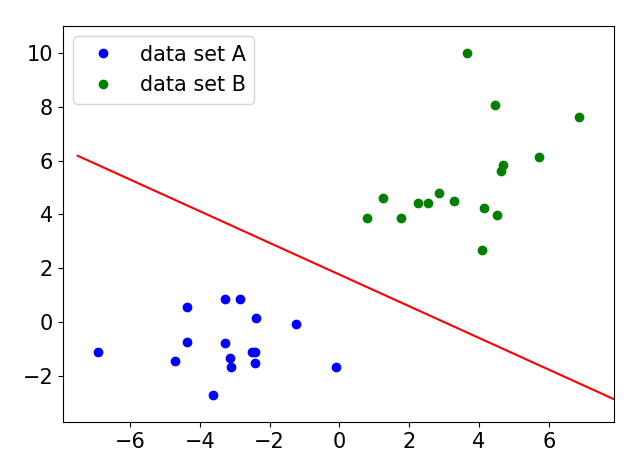
\includegraphics[width=0.6\textwidth]{gaussian_without_noise.png}
		% \centerline{\epsfig{figure=gaussian_without_noise.png,width=8.5cm}}
		%   \vspace{1.5cm}
		\centerline{(a) two disjoint gaussian samples}\medskip
	\end{minipage}
	%
	\begin{minipage}[h]{1.0\linewidth}
        \centering
        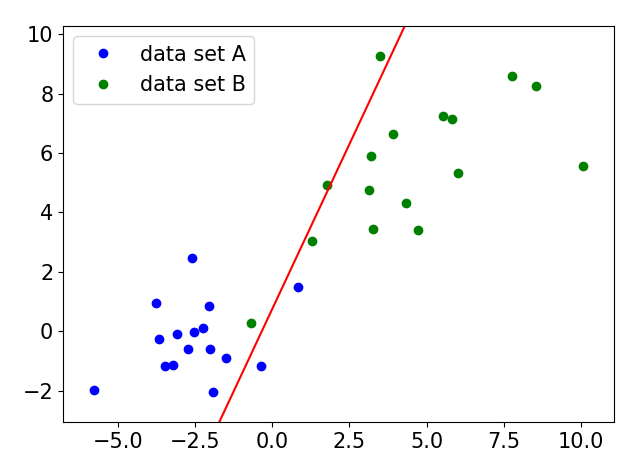
\includegraphics[width=0.6\textwidth]{gaussian_with_noise.png}
		% \centerline{\epsfig{figure=gaussian_with_noise.png,width=8.5cm}}
		%	  \vspace{1.5cm}
		\centerline{(b) two gaussian samples with a little intersection}\medskip
	\end{minipage}
	\hfill
	\begin{minipage}[h]{1.0\linewidth}
        \centering
        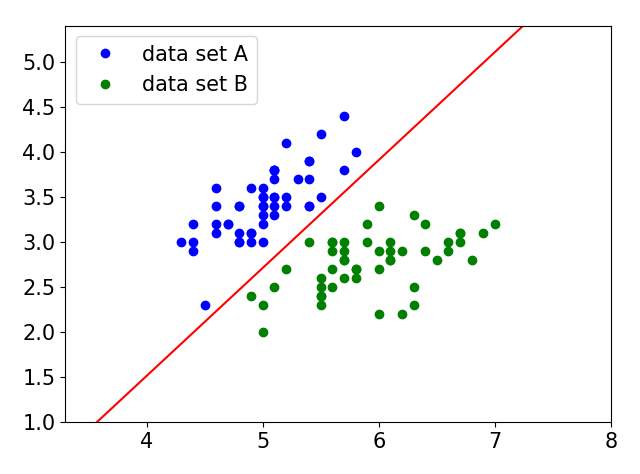
\includegraphics[width=0.6\textwidth]{another_data_set.png}
		% \centerline{\epsfig{figure=another_data_set.png,width=8.5cm}}
		%	  \vspace{1.5cm}
		\centerline{(c) datasets in python sklearn library}\medskip
	\end{minipage}
	%
	\caption{Three experimental results for linear separator.}
	\label{fig:experimental}
\end{figure}
In this section, we show three linear separation results. Result (a) and (b) in figure~\ref{fig:experimental} are
using bivariate gaussian distributions where:

\[
	\mu_A=\begin{bmatrix*}[r]
		-2 & 0
	\end{bmatrix*}\qquad
	\sigma_A=\begin{bmatrix*}[r]
		3 & 1 \\
		1 & 2
	\end{bmatrix*}
\]
and
\[
	\mu_B=\begin{bmatrix*}[r]
		4 & 5
	\end{bmatrix*}\qquad
	\sigma_B=\begin{bmatrix*}[r]
		4  & 2 \\
		2 & 3
	\end{bmatrix*}
\]
Result (a) shows our separator can separate two disjoint sets accurately. Result (b) shows even the data sets have a little intersection, our 
separator still behaves
well. Result (c) comes from iris dataset in the python sklearn library.
% \section{To be done}
% find linear separator test base to test your idea\par
% test if SVM can separate two not-disjoint set\par
% If you take interior point $x_0$ of convex hull of $A-B$ then your $A-B+x_0$ will contains 0 as interior point\par
% if set A and B are in the same hyperplane and disjoint, $p_C(x_0)$ may be $\infty$\par
% compare kernel method of SVM and transformation of your $A-B+x_0$\par
\section{Discussions}

We notice that if $A$ and $B$ are disjoint set, then $Conv(A\ominus B)$ will not include origin. Conversely, if $A$ and $B$ are not disjoint, $Conv(A\ominus B)$ 
always contains origin.
This observation holds even if we apply a nonlinear feature map on data set. It encourages us to find a new method to test if two sets are disjoint after 
applying
a nonlinear feature map.\par
% By equation \eqref{gamma bound}, we guess $\gamma$ is
% dominated by \emph{closest pair $(a,b)$ in some measure based on direction of $\ell(a-b)$}. From picture on different enlarge step, the range of $\gamma$
% keeps small and not change a lot. But small enlarge step makes equation of section 4.5 `sharper'. We guess $\ell(x_0)$ is optimal for separation problem,
% since larger convex hull indicate $p_C(x_0)$ close to 1.\par

% For set A and set B, all points of A are in the same plane, so does points in B.\par
% \emph{observation.} Enlarging convex hull will decrease alpha and increase beta. Gamma will be more close to 0
Considering analysis in section~\ref{sec:bounds analysis}, a reasonable guess is in $d$ dimensional space the minimum of $f(k_0,k_1,\cdots,k_{d-1})$ has the similar
form with equation \eqref{eq:min of f(k)}, if we know the equation of hyperplane which the vector $x_0+x_1+\cdots+x_{d-2}$ crosses. Then our separator can 
be used in
$d$ dimensional space.\par

Our code implementation computes $Conv(A\ominus B)$ by computing convex hull of $A\ominus B$. For computing convex hull in two dimensional space, the
classical algorithm Graham's scan costs $O(n\lg{n})$ time, and a better algorithm Jarvis's
march costs $O(nh)$ time, where $h$ is the vertices of convex hull~\cite{cormen2009introduction}. The prune-and-search algorithm of Kirkpatrick and Seidel
uses $O(n\lg{h})$ time~\cite{Kirkpatrick:1986:UPC:13535.13555}. \par
However, the size of $A\ominus B$ is $O(nm)$ if the size of $A$ and
$B$ are $O(n)$ and $O(m)$. If we compute $Conv(A\ominus B)$ from $Conv(A)$ and $Conv(B)$, the time complexity will decrease significantly.
Guibas and Seidel give an algorithm that computing $Conv(A\ominus B)$ in $O(n_A+m_B+c)$ time in three dimensional case, where $n_A$ and $m_B$ are the number of 
vertices of
$Conv(A)$ and $Conv(B)$, and $c$ is the number of vertices of $Conv(A\ominus B)$~\cite{Guibas:1986:CCR:10515.10525}. A similar algorithm for higher 
dimensional space will help
to decrease computing time in higher dimensional space.\par

\bibliographystyle{plain}
\bibliography{functionalapproach}

\end{document}
